However, one should note that there are many node pairs with no common neighbors. A simple way to skip over such node pairs is to start from a given vertex i, only compute similarity score between second order neighbors of i, i.e., with vertices that are neighbors of the immediate neighbors of i. Further, to speed up the process of finding common neighbors between such pairs of vertices (i.e., between the given vertex i and its second order neighbors), one many simple count the number of times each second order neigbor is reachable (with a depth first search traversal), using a data structure, such as a hashtable (with keys as the ids of the second order neighbors, and values as the count of number of the the second order neighbor has been visited / is reachable). If the similarity metric does not require the count of the common neighbors, but rather a function applied to each common neighbor, then the function can be computed and accumulated in the hashtable value (with the second order neighbor id as the associated key). Now describe our hashtable. This significantly speeds up the similarity scroe computation. Further, as there are a large number of node pairs, one may use a min-heap to keep track of the top-k edges with the highest similarity score. As an optimization, one may convert the prediction list to a heap only after X edges have been predicted.

i less than k.

To parallelize this algorithm, we partition the graph between threads, and process each partition independently on each thread (i.e., each thread has its own set of given source vertices). The best solution is to simple use dynamic schedule instead of static scheduling, with a chunk size of 2048. Each thread can now use its own hashtable, and its own perdiction-list. Since it is possible that one thread has all the top-k predicted links globally, we must use prediction lists on size k on each thread. Finally, after top-k threads have been predicted per thread. We can sort them by score, and merge them into a global top-k prediction list using a heap (mention the approach here). We also tried parallel sort, but found this approach to be more performant. We call this approach as the standard approach.

\begin{figure*}[hbtp]
  \centering
  \subfigure[Standard approach]{
    \label{fig:about-pruning--01}
    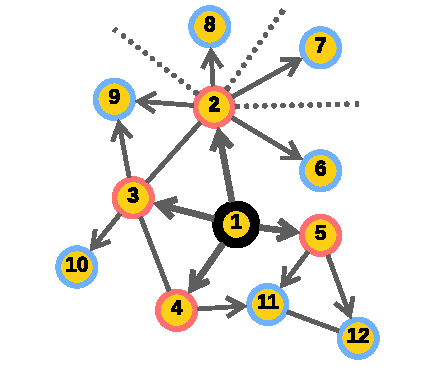
\includegraphics[width=0.31\linewidth]{out/about-pruning-01.pdf}
  }
  \subfigure[Disregard hubs with degree $> 8$]{
    \label{fig:about-pruning--02}
    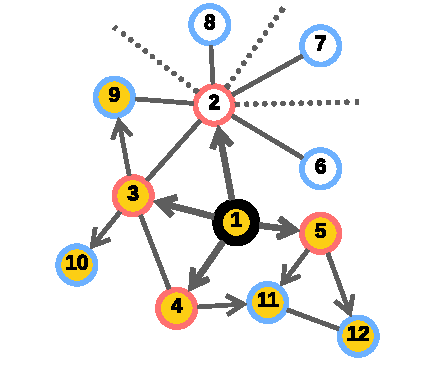
\includegraphics[width=0.31\linewidth]{out/about-pruning-02.pdf}
  }
  \subfigure[Disregard hubs with degree $> 4$]{
    \label{fig:about-pruning--03}
    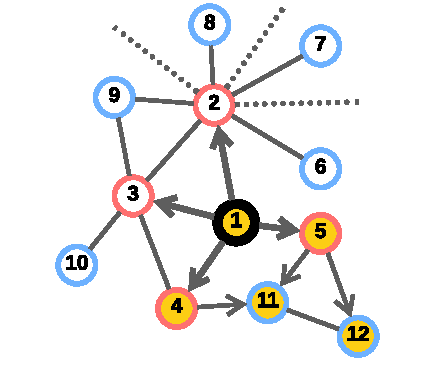
\includegraphics[width=0.31\linewidth]{out/about-pruning-03.pdf}
  } \\[-2ex]
  \caption{Illustration of our neighborhood-based link prediction approach, which disregards large hubs (first-order neighbors with high degree). The approach applies to each vertex in the graph. Here, we focus on the neighborhood of a vertex $1$ in the graph. The current vertex $1$ is outlined in black, its first-order neighbors in red, and its second-order neighbors in blue. Edge directions indicate traversal, with some second order vertices omitted for simplicity (dotted edges). (a) Depicts the standard approach, which considers all second-order neighbors of vertex $1$. (b) Presents our approach, which considers only second-order neighbors linked to $1$ through a small hub (degree $\leq 8$). This pruning reduces runtime and enhances prediction quality. (c) Illustrates our approach, where vertices with degree $> 4$ are considered large hubs.}
  \label{fig:about-pruning}
\end{figure*}

\begin{figure}[hbtp]
  \centering
  \subfigure{
    \label{fig:about-hashtable--all}
    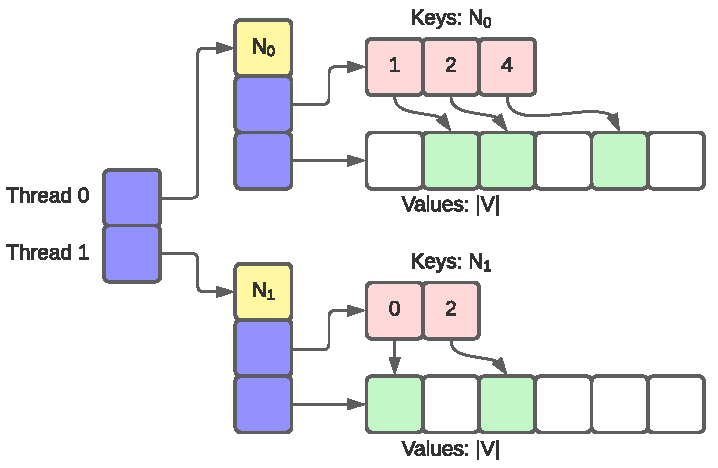
\includegraphics[width=0.88\linewidth]{out/about-hashtable.pdf}
  } \\[-2ex]
  \caption{Illustration of collision-free per-thread hashtables that are well separated in their memory addresses, for two threads. Each hashtable consists of a keys vector, a values vector (of size $|V|$), and a key count ($N_0$/$N_1$). The value associated with each key is stored/accumulated in the index pointed by the key. As the key count of each hashtable is updated independently, we allocate it separately on the heap to avoid false cache sharing \cite{sahu2023gvelouvain}. These are used in the scoring phase of our implementation to track common neighbors.}
  \label{fig:about-hashtable}
\end{figure}


\ignore{How do you explore the neighbors of each node, and compute intersection? What is a super naive way to do the above?}

- Explain NetworKit, too bad crash. \\
- Explain the Naive approach (where max mediator degree is $\infty$). \\
- Explain our approach with diagram.

\ignore{Are there no missing links in the original graphs?}

\ignore{Runtime + speedup + precision for $0.1|E|$.
Lu et al. \cite{lu2015toward} use precision.}

\ignore{What is the expected precision of random guess?}

\ignore{Why the choice of best method appears to change with batch size?}

\ignore{How do you maintain per-thread prediction list? Is it efficient? How do you merge the prediction lists? Is it efficient?}

\ignore{Explain the detailed detailed approach diagram. How do you explore reachable nodes at distance 2. How do you compute intersection (or score for AA, RA)? How do you skip high-degree mediators (or 1st order neighbors)? Why is this efficient?}

\ignore{Results are not deterministic - why? Because multiple matching scores (like MST).}

\ignore{We now avoid self-loops and first order neighbors.}

\ignore{We fixed adamic adar and resource allocation metrics.}

\ignore{We managed per-thread scoring heap properly (maxheap), using suitable popback, pushback, back.}

\ignore{We used heap for merging phase instead of parallel sort with resize/trim to avoid OOM issue.}

\ignore{We added common neighbors metric.}

\ignore{We removed self-loops from the graphs.}

\ignore{We sort tuples naturally.}


Illustration our our approach of neighborhood-based link prediction, where we disregard large hubs (i.e., first order neighbors with high degree). Here, we consider the neighborhood of vertex $1$ in the graph, where the current vertex, i.e., $1$ is shown with a black border, its first order (immediate) neighbors are shown with a red border, and its second order neighbors are shown with a blue border. The direction of the edges indicate the direction of traversal, and $3$ neighbors of vertex $2$ are not shown (dotted edges) for figure simplicity. (a) Shows the standard approach, where all the second order neighbors of the current vertex $1$ are considered, i.e., vertices $6$, $7$, $8$, $9$, $10$, $11$, and $12$. (b) Shows our approach, where only the second order neighbors linked to vertex $1$ by a small hub with degree lower than or equal to $8$, i.e., vertices $9$, $10$, $11$, and $12$ linked to $1$ through $3$, $4$, and $5$, are considered. This is based on the intuition that vertices with low degree confer significant similarity among their neighbors, while vertices with high degree do not (i.e., they confer little similarity among their neighbors). This pruning provides a significant reduction in runtime of the link prediction algorithm, while also improving the quality of the predictions. Note that second order neighbors of $1$ can still be considered, but only if they are also linked to $1$ by a small hub (such as vertex $9$, which is also linked to $1$ through $3$). Finally, (c) shows our approach, where only the second order neighbors linked to the current vertex by a small hub with degree lower than or equal to $4$ are considered (i.e., vertices $11$ and $12$ linked to $1$ through $4$ and $5$) --- in other words, vertices with degree higher than $4$ as considered large, and thus second order neighbors of $1$ connected to such a hub are disregarded. Note that the figure shows the neighborhood of vertex $1$ only, but the same approach is applied to all vertices in the graph.

% Low degree vertices, such as $2$, confer significant similarity among its neighbors, while high-degree vertices, such as $3$, do not. Here $4$ is a second-order neighbor of $1$.

% This figure illustrates our approach for minimizing the exploration for second degree neighbors of a given for computing neighbor-based similarity scores. The core of our idea is that a node (which a first order neighbor of the given node) with a high degree, i.e., a hub, does not confer significant similarity among its neighbors. However, if a node has low degree, its neigbors are likely to be similar to each other. Based on this idea, if the first order neighbor (or simply neighbor) of the given node has high degree (i.e., degree greater than max mediator degree), we simply skip exploring the second order neighbors from such a high degree node. This in fact significantly improves the performance of the scoring phase, even though the works case complexity of the algorithm is still the same.

% In the above figure, we show a region of a graph, which has 16 vertices. Here, 1 is the given vertex. By default, we explore the first order neighbors of 1 with DFS (the first order neighbors of vertex 1 are marked red border). From each first order neighbor, i.e., from 2, 3, 4, and 5, we explore the second order neighbors of vertex 1, i.e., vertices 6, 7, 8, 9, 10, 11, 12. For each second order neighbor $k$, we increment the hashtable value for $k$. This effectively allows us to obatin $|\Gamma_i \cap \Gamma_k|$ for each second order neighbor of vertex 1 in the hashtable. This is then used to compute the similarity score of each vertex with its second order neighbors. As the graph is undirected, we skip second order neighbors, where the id of the second order neighbor is less than or equal to the given vertex $i$. The scores are the added to a list. The process repeats for each vertex in the graph.

% In the second part of the figure, we show the case with max mediator degree 8 and 4. Explain this later.




\subsection{Optimizations for Local Neighborhood-based Similarity search}
\label{sec:leiden}

Consider an undirected graph $G(V, E)$. For each vertex $u$ in the graph, we count the number of paths to each second order neighbor of $u$, i.e., we calculate $N(u) \cap N(w)$ for each $w \in N(N(u))$. We then use this to calculate two different neighbor similarity metrics, namely, Jaccard's coefficient (JC) and Hub-Promoted (HP) score \cite{gatadi2023lpcd}. By \textit{exploring only second order neighbors} of each vertex, we skip computing scores on pairs of vertices which have no neighbors in common, and thus have a similarity score of $0$. We parallelize this approach with OpenMP's \textit{dynamic} schedule, with a chunk size of $2048$, and optimize path counting and lookup with per-thread collision-free hashtables. Note that we only want to predict links between node pairs with top-$k$ similarity scores, with $k$ being a fraction of the number of edges in the original graph $|E|$. Accordingly, we use a per-thread min-heap based prediction list, which allows us to keep node pairs with top-$k$ scores (per thread), and evict the node pair with the lowest score once we have a node pair with a higher score. Once all vertices have been processed by the threads, we concatenate the prediction lists, sort them by similarity score in increasing order, and return only the top-$k$ links predicted. As an optimization, we convert the per-thread prediction lists into a min-heap only when the prediction lists is populated with $k$ entries. At this stage, predicting links on graph with $2.3$ million edges using $24$ threads takes $14$ seconds.

To further optimize link prediction, we note that low-degree nodes are users who have only a few connections in the social network. These users are more selective in accepting friend requests and are likely to form connections with people they have stronger, more meaningful relationships with, such as close friends and family. Thus, low-degree nodes confer significant similarity among their neighbors, while high-degree nodes generally do not (due to their lack of selectivity). Accordingly, for vertex $u$, we only explore neighbors of $v \in N(u)$ only if $degree(v) \leq D$ (where $D$ is the degree threshold for a neighbor of $u$). With $D = 4$, predicting links on the $2.3$ million edge graph\ignore{ using $24$ threads} now takes only $10$ milliseconds. Figure \ref{fig:about-pruning} shows an explanation of this approach. Here, vertex $4$ is considered for similarity score calculation with vertex $1$, as they are both linked to a common low-degree neighbor, i.e., vertex $2$. However, neighbors of high-degree vertex $3$ are not considered for score calculation.

\ignore{What does precision mean in the plots? \% of matching links with ground truth? How many ground truth links were missed?}

\ignore{Explain the confusion y-axis on precision.}

\ignore{All approaches require computing intersection, or intersection-like, even AA and RA.}

\ignore{On a set of smaller graphs, we observe/identify the most precise approaches, and observe the X, X, and X to perform the best. Accordingly, we run these methods on the graphs in our dataset.}

\ignore{Comparison with baseline approach ($\infty$), i.e., exploring all possible/reachable pairs at distance 2, and quickly computing intersection, scores, adding to heap, and merging across threads. Explain with figure in approach.}

\ignore{Why precision on road networks and protein k-mer graphs low? (low average degrees)}

% \input{src/fig-leidenopt-runtime}
% \input{src/fig-leidenopt-modularity}
% \input{src/fig-leiden-pass}




\subsection{Our DLH implementation}

We now explain the psuedocode our approach for parallel neighborhood-based link prediction, which disregards large hubs (DLH), which is given in Algorithm \ref{alg:predict}. Here, the \texttt{predictLinks} function accepts the input graph $G$, the maximum number of edges to predict $N_P$, a minimum score $S_{min}$, and outputs a list of predicted edges $P$. The algorithm operates in two main phases: the scoring phase and the merging phase.

In the \textit{scoring phase} (lines \ref{alg:predict--scoring-begin}-\ref{alg:predict--scoring-end}), each vertex $i$ is processed in parallel. For each vertex, we scan its second-order neighbors, considering only neighbors of those first order neighbors which have a degree ($D_j$) less than or equal to a specified maximum degree ($\Pi_j$) --- this is based on the idea that large hubs (here, the first order neighbors) confer little similarity among its neighbors (here, between the current vertex $i$, and its second order neighbors). The scoring of potential edges is done in the \texttt{scanEdges} function (lines \ref{alg:predict--scan-begin}-\ref{alg:predict--scan-end}). Here we skip the reverse edges (where $k \leq i$), and calculate a score for each potential second order neighbor $k$ based on the given metric, i.e., for the Adamic-Adar (AA) and Resource Allocation (RA) metrics, we apply the scoring formula for each common neighbor, and for the other metrics, we simply count the number of common neighbors. The scores (or the number of common neighbors) are accumulated in a collision-free per-thread hashtable $H_t$. After scanning, we set entries corresponding to first-order neighbors of $i$ to $0$ in $H_t$ to avoid considering them as potential edges (line \ref{alg:predict--avoid-neighbors1}). We then calculates a score for each potential edge $(i, k)$ from the hashtable $H_t$, and if the score exceeds the minimum threshold $S_{min}$, the edge is added to a per-thread prediction list $P_t$. The list is maintained as a min-heap based on scores (after $N_P$ edges have been added), in order to efficiently keep track of top $N_P$ edges. The size of $P_t$ is controlled to keep only the top-scoring edges. After scoring all the vertices in parallel, the algorithm proceeds to the merging phase.

In the \textit{merging phase} (lines \ref{alg:predict--merging-begin}-\ref{alg:predict--merging-end}), the per-thread prediction lists are merged into a global prediction list $P$. This is done by first sorting the per-thread lists based on the scores. A max heap $P_h$ is then created to track the maximum score from each thread. Then we iteratively select the highest-scoring edge from the threads and adds it to the global list until either the maximum number of edges is reached $N_P$ or there are no more edges to consider (lines \ref{alg:predict--merge-loop-begin}-\ref{alg:predict--merging-end}).

\ignore{Explain the algorithm, including the baseline. Tell which parameter setting of max mediator degree is suitable.}

\begin{figure*}[hbtp]
  \centering
  \subfigure[Relative runtime (logarithmic scale), of each link prediction method]{
    \label{fig:adjust-mindegree--runtime}
    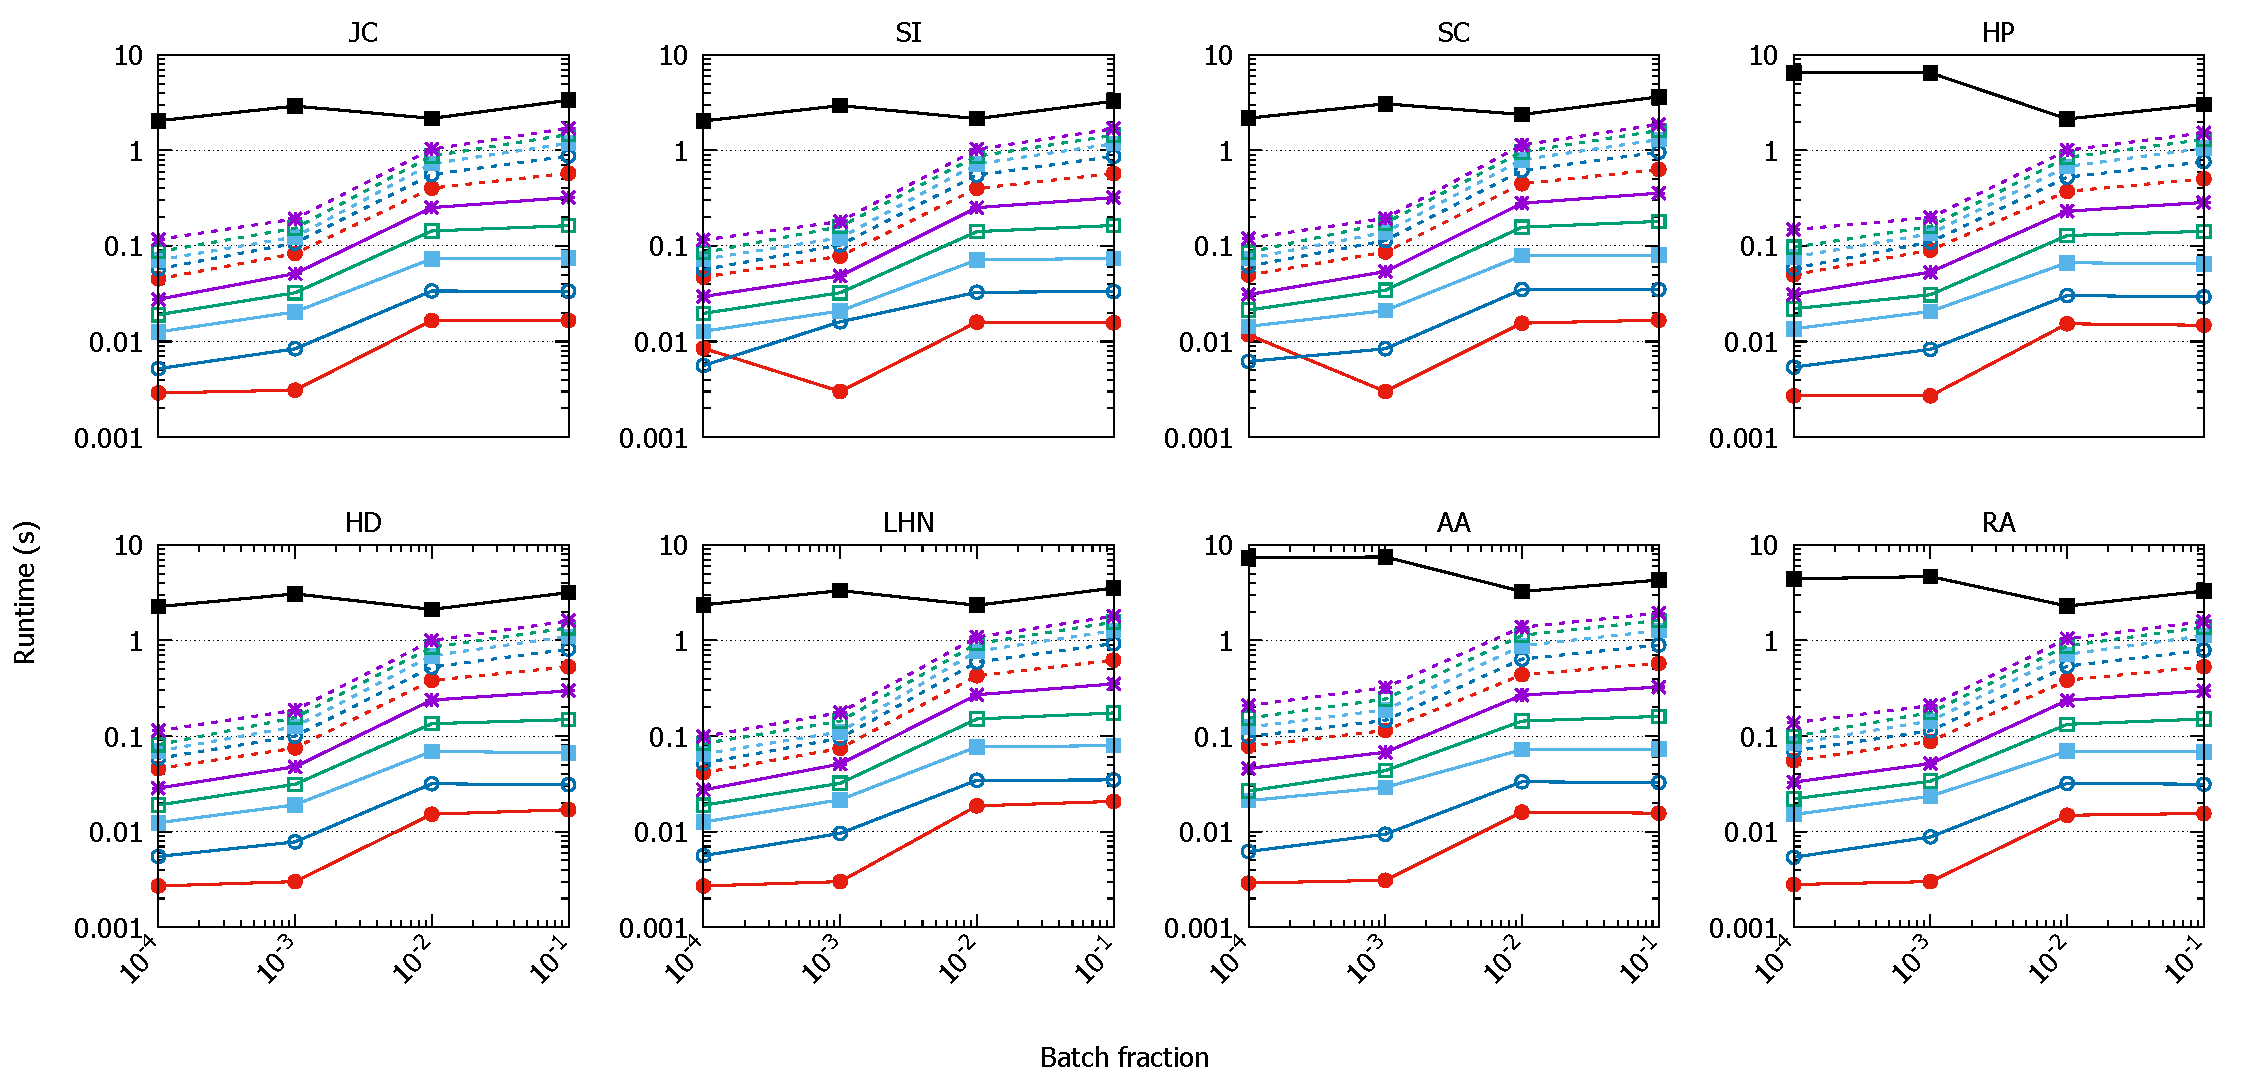
\includegraphics[width=0.98\linewidth]{out/adjust-mindegree-runtime.pdf}
  }
  \subfigure[F1 score of predicted links (logarithmic scale), of each link prediction method]{
    \label{fig:adjust-mindegree--precision}
    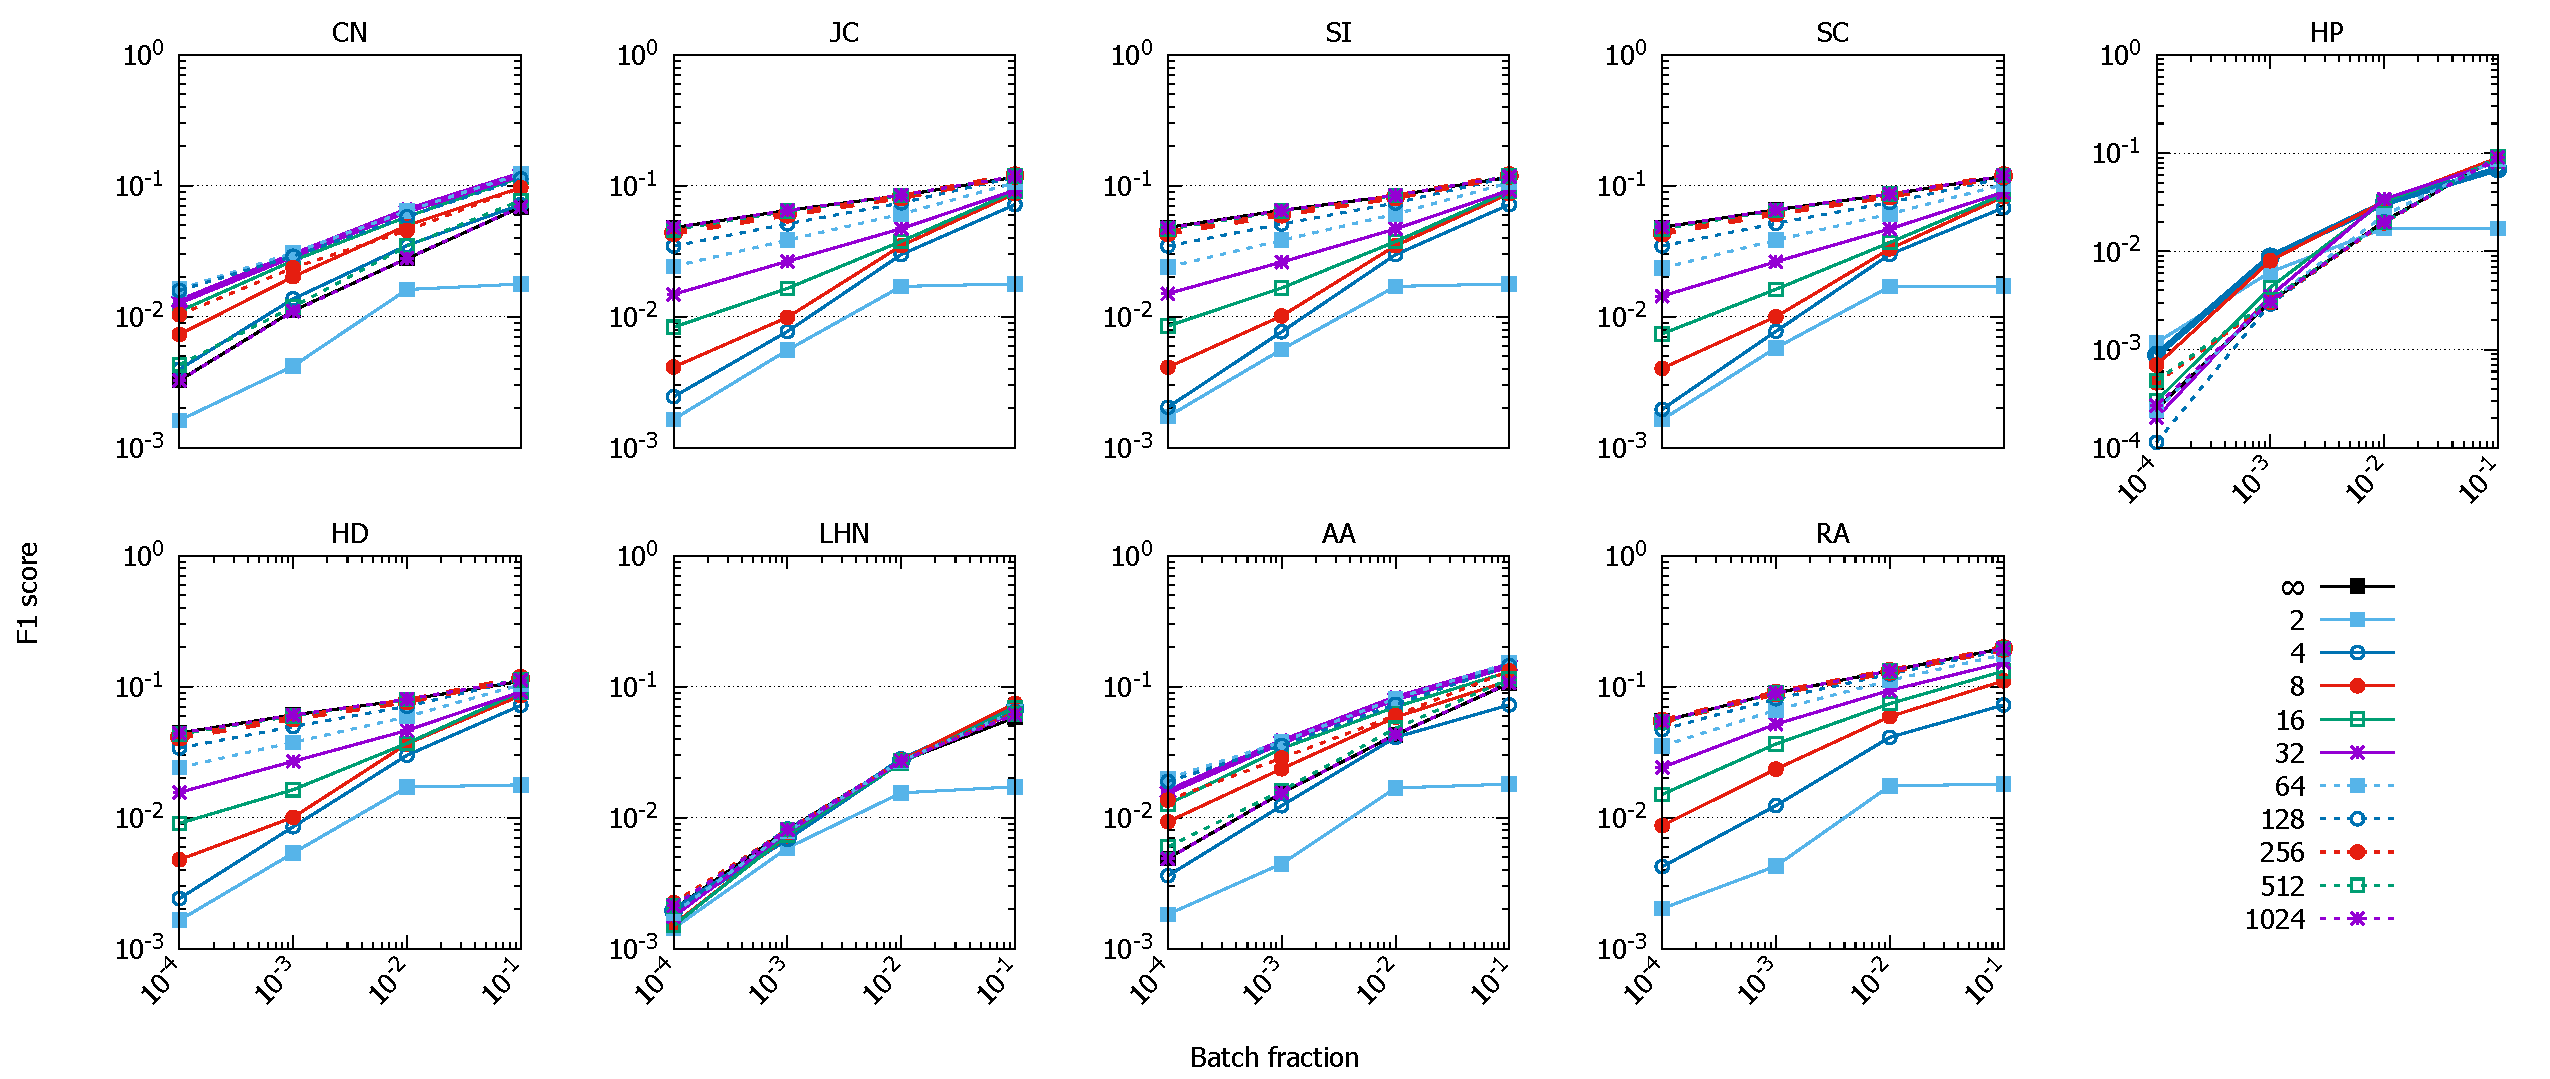
\includegraphics[width=0.98\linewidth]{out/adjust-mindegree-f1score.pdf}
  } \\[0ex]
  \caption{Impact of adjusting the \textit{MAX\_MEDIATOR\_DEGREE} from $2$ to $1024$ (in multiples of $2$), and to $\infty$, on the runtime (in seconds, log-scale), and precision of predicted links (in percentage, log scale), of each neighbor-based link prediction method, on batch sizes of $10^{-4}|E|$ to $0.1|E|$. The full form of each link prediction method is given in Section X.}
  \label{fig:adjust-mindegree}
\end{figure*}

\begin{algorithm}[hbtp]
\caption{Our Parallel \textit{Disregard Large Hubs (DLH)} approach.}
\label{alg:predict}
\begin{algorithmic}[1]
\Require{$G(V, E)$: Input graph}
\Require{$N_P$: Maximum number of edges to predict}
\Require{$S_{th}$: Threshold score above which to predict}
\Ensure{$a, b, c$: Current vertex, first-order, second-order neighbor}
\Ensure{$L_H$: Hub limit, i.e., large hub degree threshold}
\Ensure{$|\Gamma_b|$: Degree of first-order neighbor $b$}
\Ensure{$H_t$: Collision-free per-thread hashtable}
\Ensure{$P_t$: Per-thread prediction list}
\Ensure{$P_h$: Heap for merging per-thread prediction lists}
\Ensure{$P$: Global prediction list}

\Statex

\Function{predictLinksDLH}{$G, N_P, S_{th}$} \label{alg:predict--begin}
  \State $\rhd$ Scoring phase
  \State $P_t \gets \{\}$ \textbf{on each thread} \label{alg:predict--scoring-begin}
  \ForAll{$a \in V$ \textbf{in parallel}}
    \State $\rhd$ Scan second-order neighbors of $a$
    \State $H_t \gets \{\}$
    \ForAll{$b \in G.out(a)$}
      \State $\rhd$ Skip high degree first-order neighbors
      \If{$|\Gamma_b| \leq L_H$} $scanEdges(H_t, G, b)$
      \EndIf
    \EndFor
    \State $\rhd$ Avoid first-order neighbors
    \ForAll{$b \in G.out(a)$} $H_t[b] \gets 0$ \label{alg:predict--avoid-neighbors1}
    \EndFor
    \State $\rhd$ Get prediction scores and add to list
    \ForAll{$c \in H_t.keys()$}
      \State $score \gets computeScore(a, c, H_t[c])$
      \If{$score \leq S_{th}$} \textbf{continue}
      \EndIf
      \State $\rhd$ Add edge $(a, c)$ to prediction list
      \If{$|P_t| < N_P$}
        \State $P_t.push(\{a, c, score\})$
        \If{$|P_t| = N_P$} $P_t.makeMinHeapByScore()$
        \EndIf
      \ElsIf{$score \geq P_t[0].score$}
        \State $P_t.popHeap()$
        \State $P_t.pushHeap(\{a, c, score\})$
      \EndIf
    \EndFor
  \EndFor \label{alg:predict--scoring-end}
  \State $\rhd$ Merging phase \label{alg:predict--merging-begin}
  \State $P \gets \{\}$ \textbf{;} $P_h \gets \{\}$
  \State $sort(P_t)$ \textbf{on each thread}
  \ForAll{$t$ in threads}
    \If{$|P_t| \neq 0$} $P_h.push(\{t, P_t.back().score\})$
    \EndIf
  \EndFor
  \State $P_h.makeMaxHeapByScore()$ 
  \While{$|P_h| \neq 0$ \textbf{and} $|P| < N_P$} \label{alg:predict--merge-loop-begin}
    \State $t \gets P_h.popHeap().t$
    \State $P.push(P_t.back())$
    \State $P_t.pop()$
    \If{$|P_t| \neq 0$} $P_h.pushHeap(\{t, P_t.back().score\})$
    \EndIf
  \EndWhile \label{alg:predict--merging-end}
  \Return{$P$}
\EndFunction \label{alg:predict--end}

\Statex

\Function{scanEdges}{$H_t, G, a, b$} \label{alg:predict--scan-begin}
  \ForAll{$c \in G.out(b)$}
    \State $\rhd$ Skip reverse edges
    \If{$c \leq a$} \textbf{continue}
    \EndIf
    \If{$metric = AA$} $H_t[c] \gets H_t[c] + 1 / log(|\Gamma_b|)$
    \ElsIf{$metric = RA$} $H_t[c] \gets H_t[c] + 1 / |\Gamma_b|$
    \Else\ $H_t[c] \gets H_t[c] + 1$
    \EndIf
  \EndFor
\EndFunction \label{alg:predict--scan-end}
\end{algorithmic}
\end{algorithm}


% For this, we adjust the degree threshold $D$ from $4$ to $32$ in multiples of $2$.

% This figure illustrates our approach for minimizing the exploration for second degree neighbors of a given for computing neighbor-based similarity scores. The core of our idea is that a node (which a first order neighbor of the given node) with a high degree, i.e., a hub, does not confer significant similarity among its neighbors. However, if a node has low degree, its neigbors are likely to be similar to each other. Based on this idea, if the first order neighbor (or simply neighbor) of the given node has high degree (i.e., degree greater than max mediator degree), we simply skip exploring the second order neighbors from such a high degree node. This in fact significantly improves the performance of the scoring phase, even though the works case complexity of the algorithm is still the same.

% In the above figure, we show a region of a graph, which has 16 vertices. Here, 1 is the given vertex. By default, we explore the first order neighbors of 1 with DFS (the first order neighbors of vertex 1 are marked red border). From each first order neighbor, i.e., from 2, 3, 4, and 5, we explore the second order neighbors of vertex 1, i.e., vertices 6, 7, 8, 9, 10, 11, 12. For each second order neighbor $k$, we increment the hashtable value for $k$. This effectively allows us to obatin $|\Gamma_i \cap \Gamma_k|$ for each second order neighbor of vertex 1 in the hashtable. This is then used to compute the similarity score of each vertex with its second order neighbors. As the graph is undirected, we skip second order neighbors, where the id of the second order neighbor is less than or equal to the given vertex $i$. The scores are the added to a list. The process repeats for each vertex in the graph.

% In the second part of the figure, we show the case with max mediator degree 8 and 4. Explain this later.


%% NOTE; What is the complexity of each similarity metric. Mention at the end of all in preliminaries.
